\newpage
\subsection{Messages Page}

%For the main pages put a mockup and describe it in detail.

%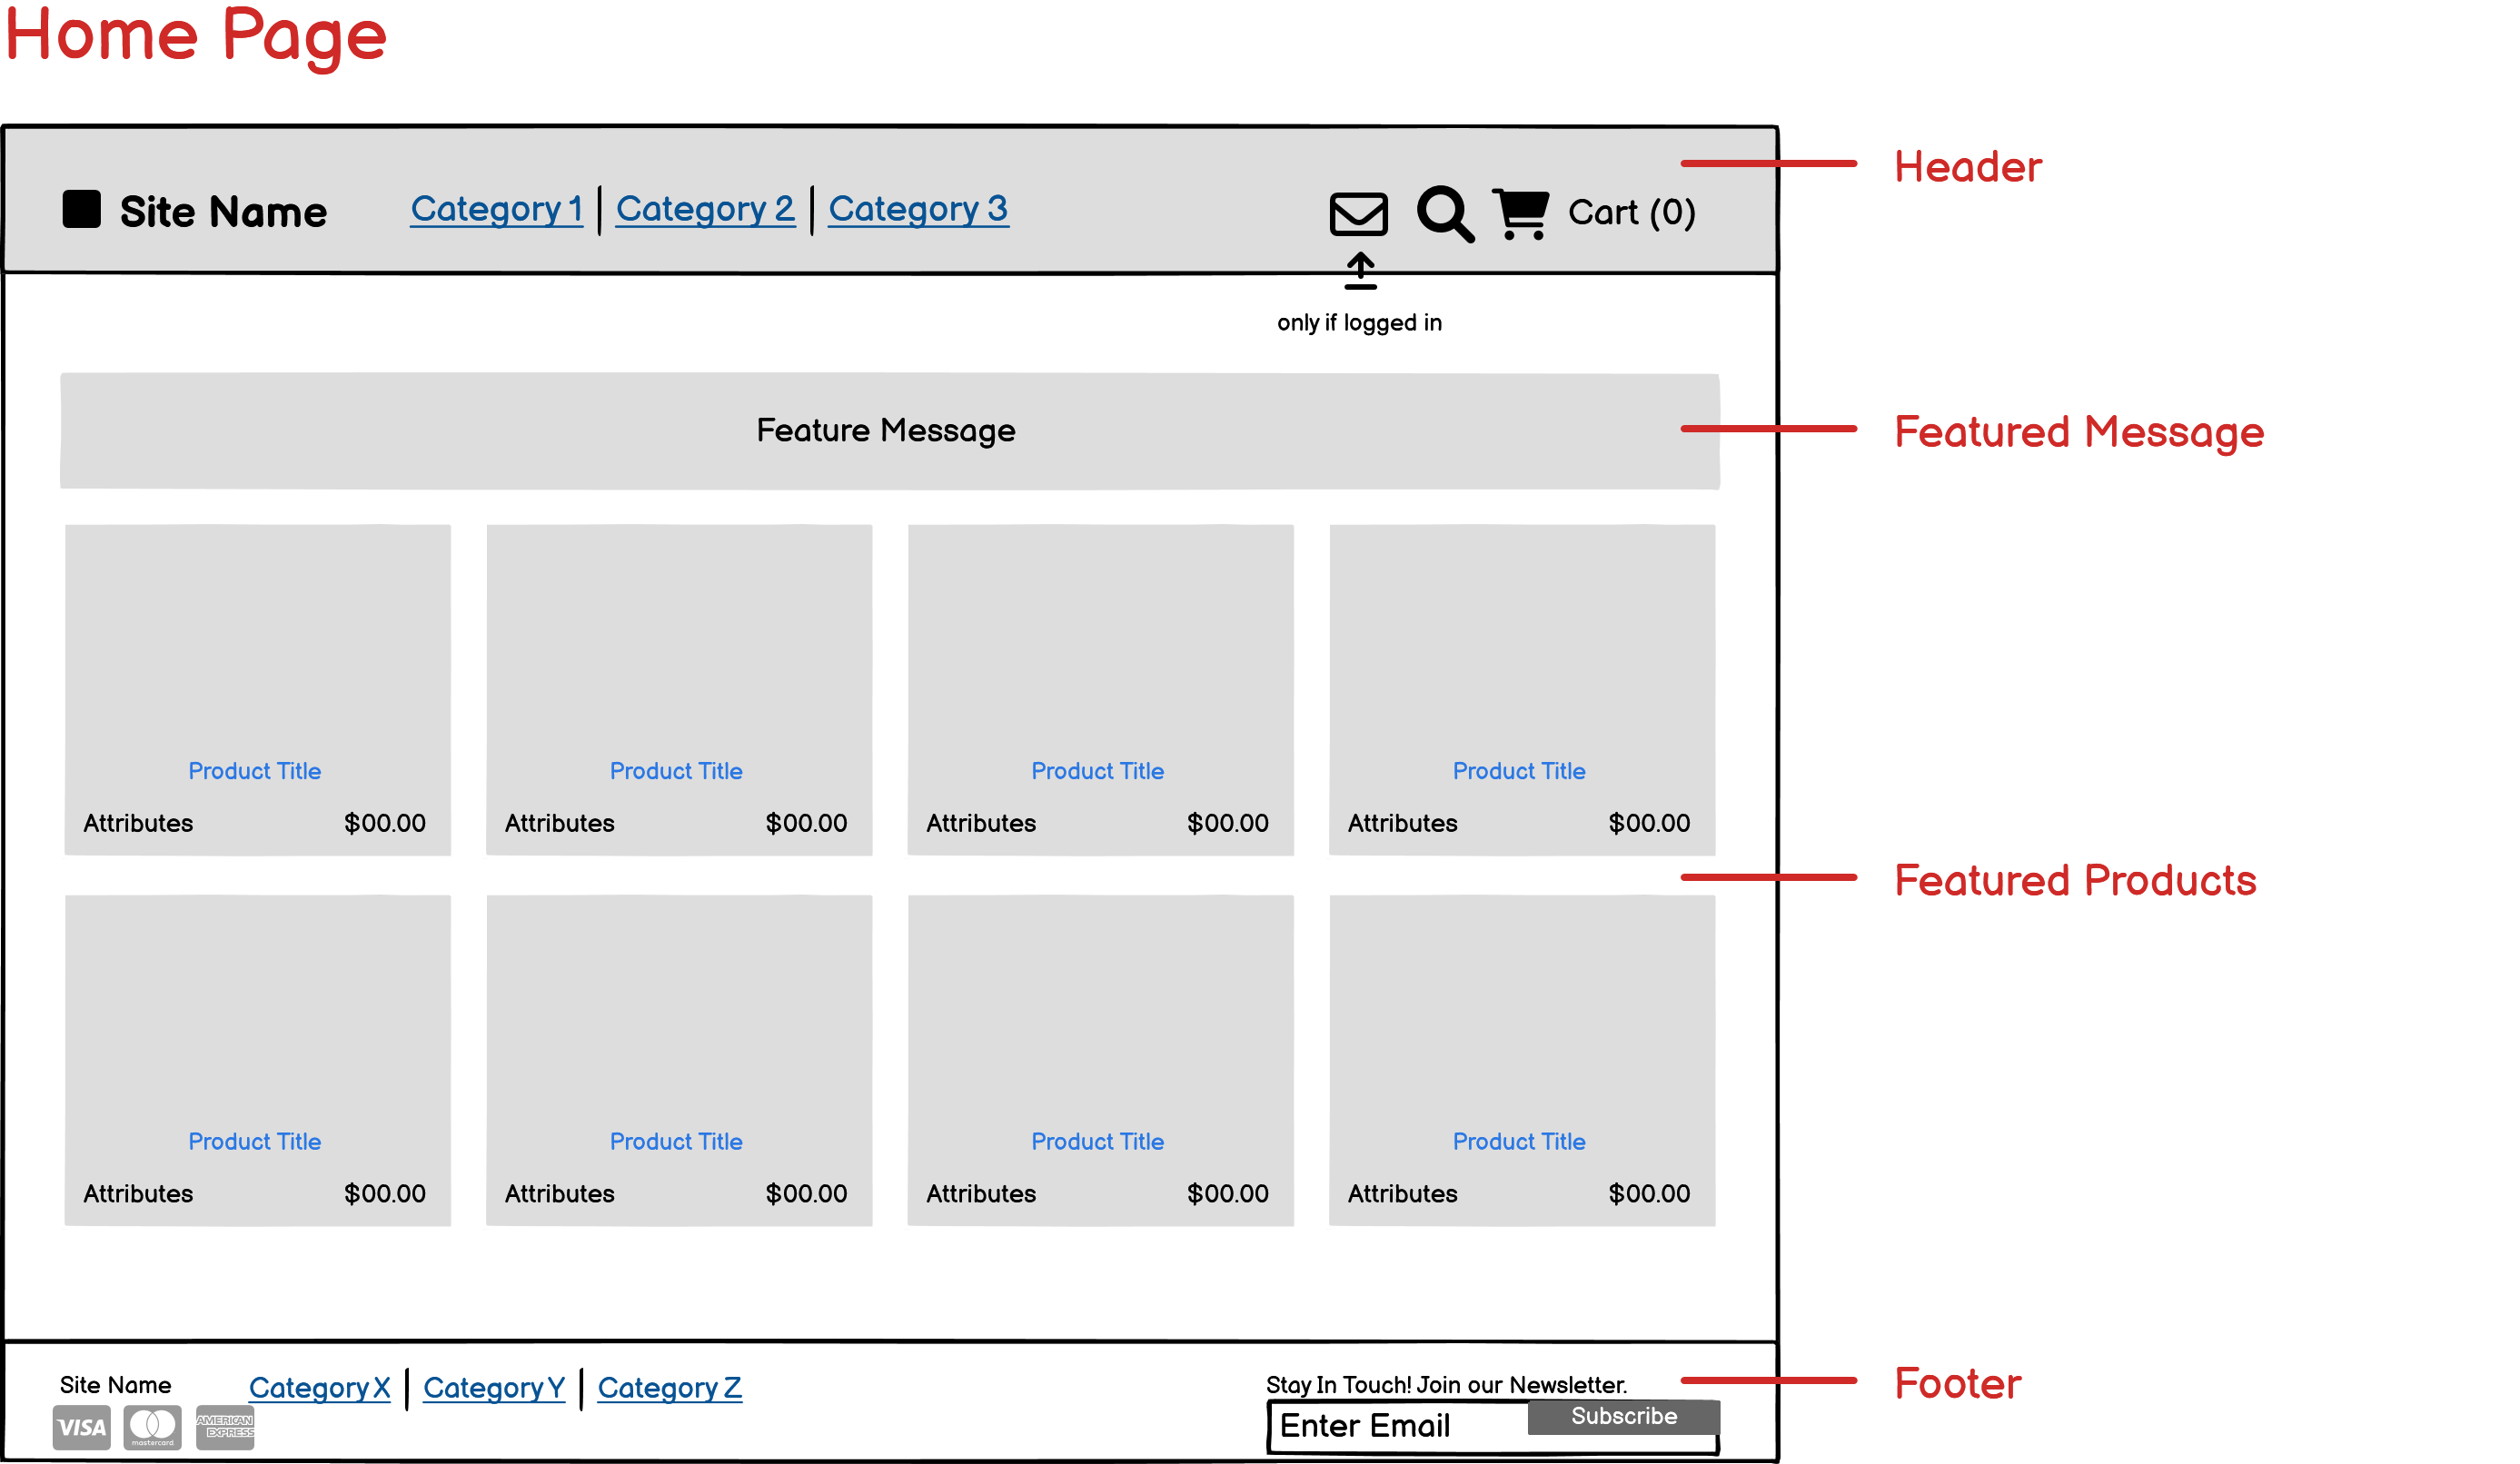
\includegraphics[scale=0.5]{logos/Images/pages/Home Page.png}

\begin{figure}[h]
    \centering
    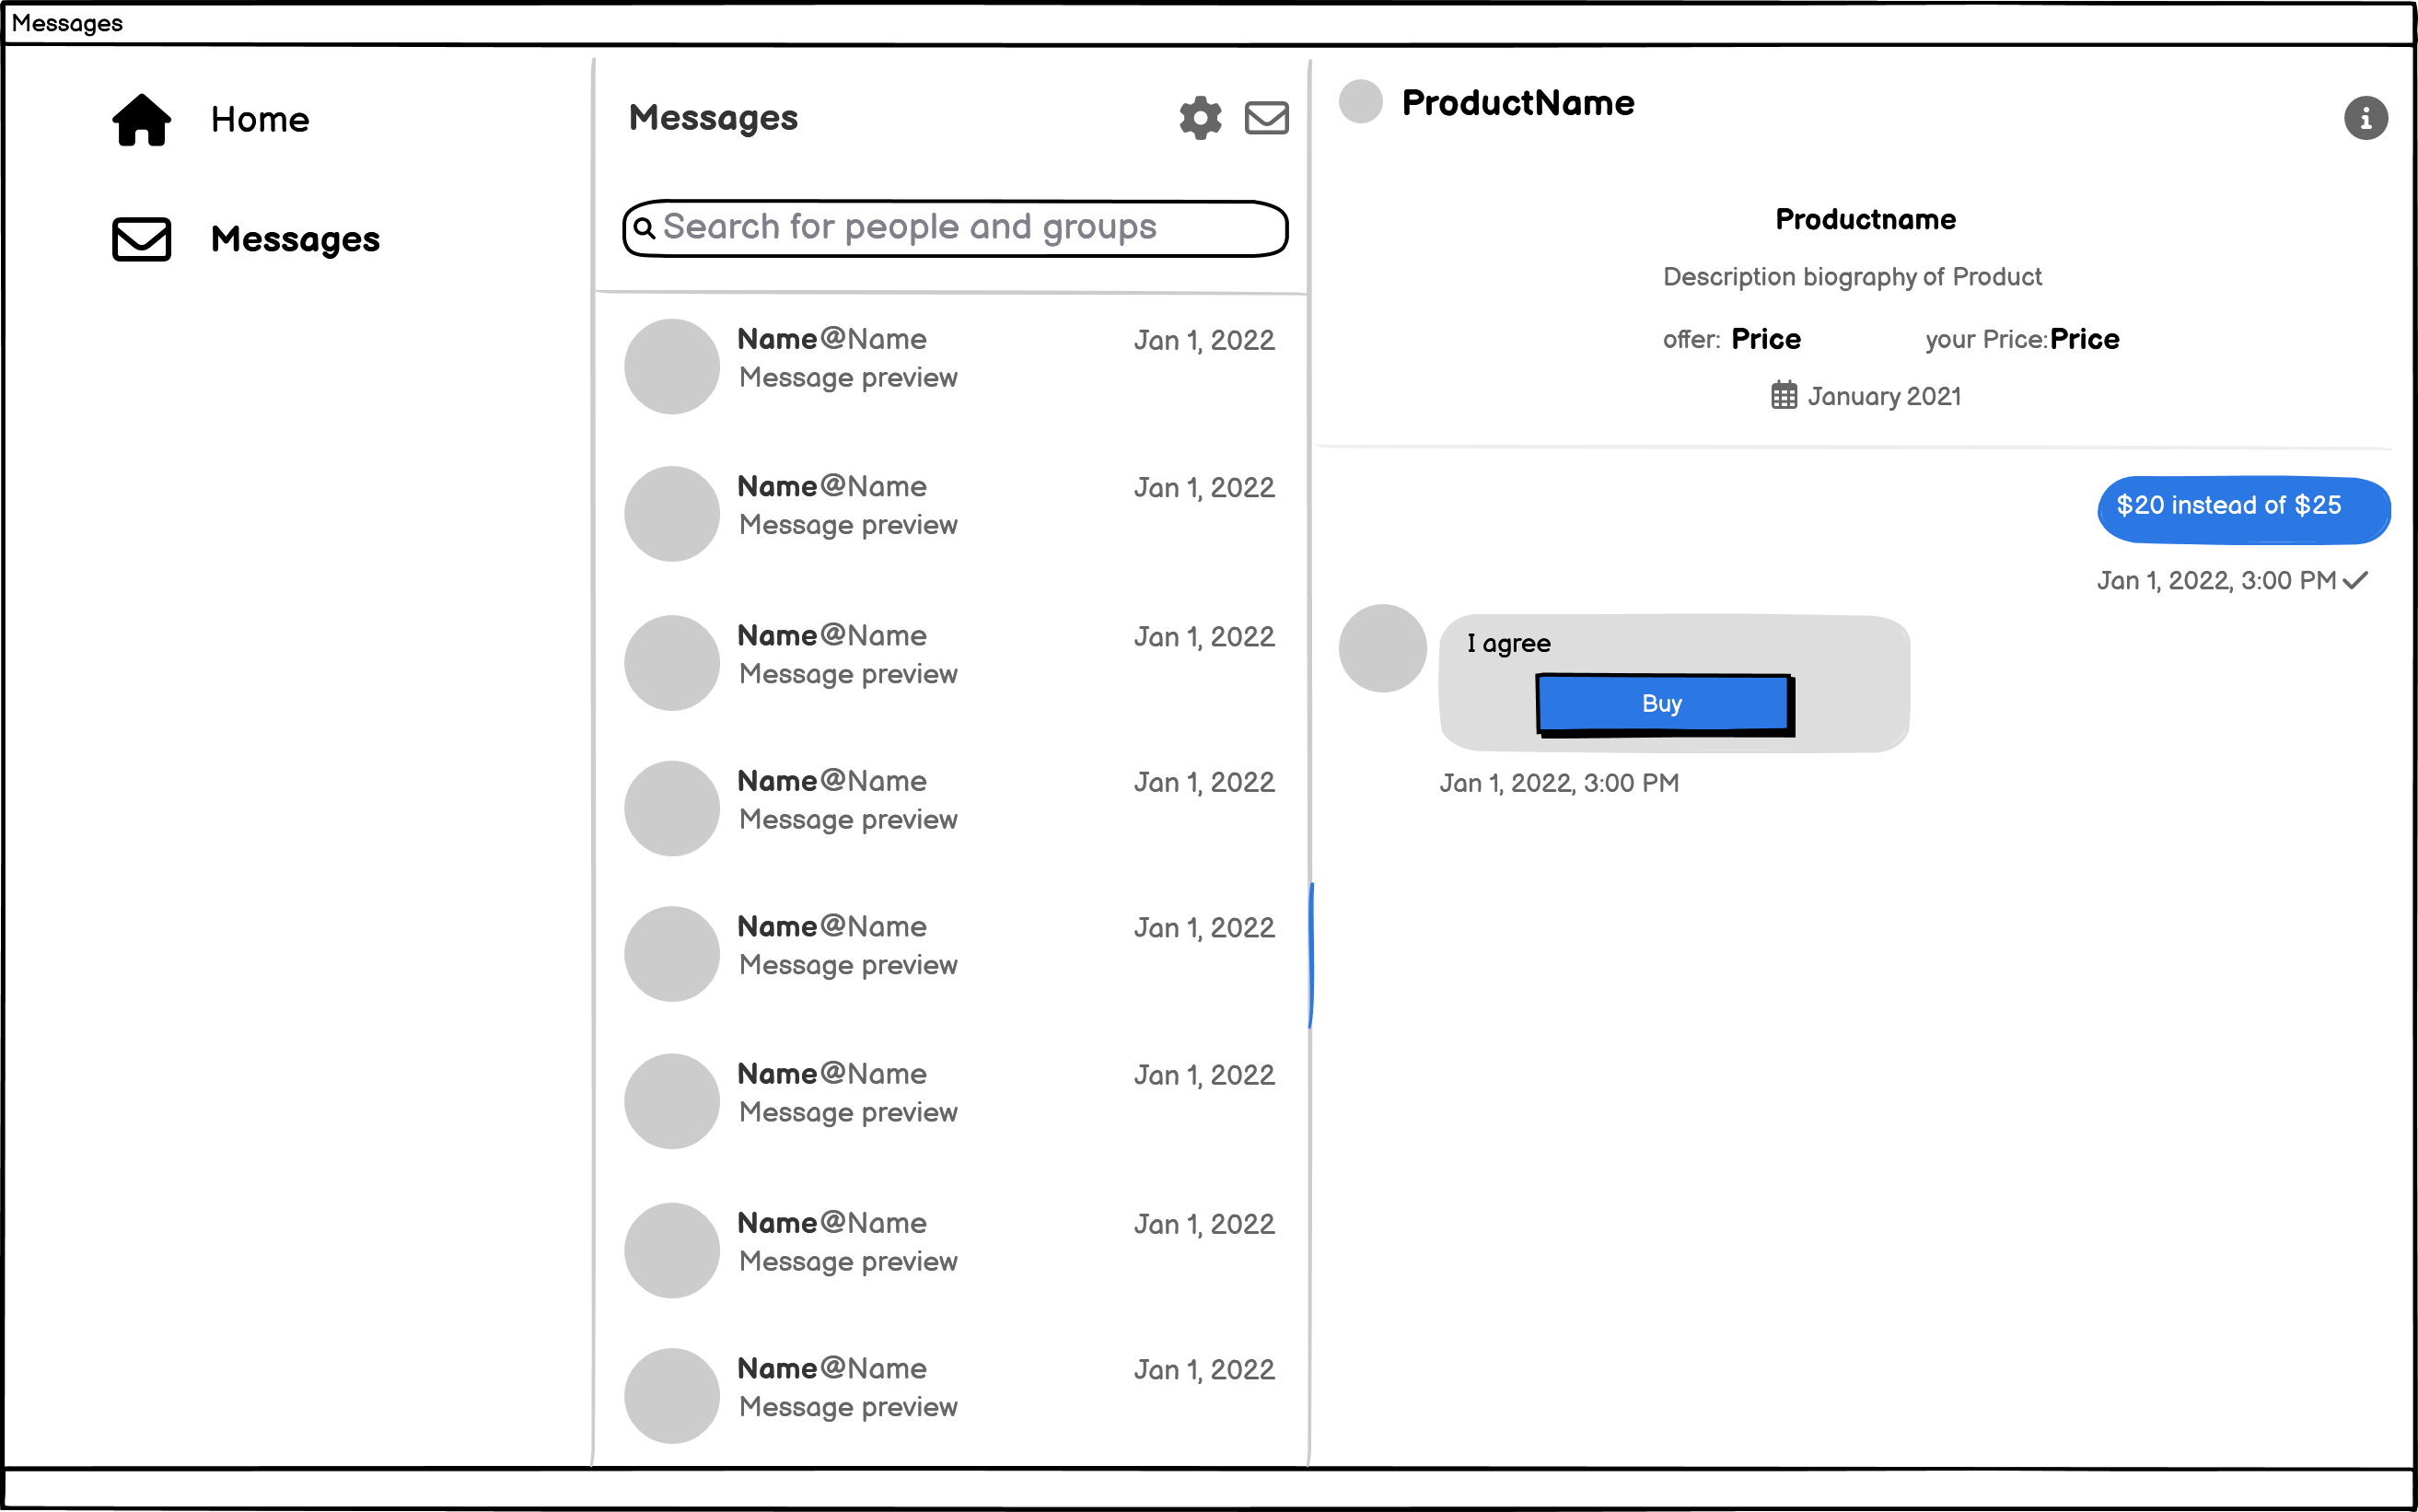
\includegraphics[scale=0.45]{logos/Images/pages/Messages.png}
    \caption{Messages Page}
    \label{fig:my_label}
\end{figure}
\hfill \break
On this website potential buyers have the opportunity to buy products. If they find a product they like but the price is too high, there is a possibility to make a counteroffer to the seller.\\\\
If a buyer wants to make a counteroffer, they can specify a new price and send a message to the seller explaining and justifying the offer. The seller is then informed of the message and can either accept or reject the offer.\\\\
If the seller accepts the offer, the buyer can buy the product at that price. If the seller rejects the offer, the buyer can either buy the product at the original price or make a new offer.\\\\
In our example, the seller is supposed to agree to the buyer's offer. Once the buyer has made an offer, the seller will receive a message with the buyer's offer. The seller can then accept the offer by sending a message to the buyer accepting the offer and discussing further details on how to pay and ship the product.\\\\
Overall, this site provides a simple and reliable way for buyers to make counteroffers and for sellers to accept or reject those offers. Using messaging as a means of communication ensures that buyers and sellers can stay in touch and find an amicable solution if the original price is not acceptable.